% Created 2019-06-21 ven. 14:11
\documentclass{article}
\usepackage[utf8]{inputenc}
\usepackage[T1]{fontenc}
\usepackage{fixltx2e}
\usepackage{graphicx}
\usepackage{longtable}
\usepackage{float}
\usepackage{wrapfig}
\usepackage{rotating}
\usepackage[normalem]{ulem}
\usepackage{amsmath}
\usepackage{textcomp}
\usepackage{marvosym}
\usepackage{wasysym}
\usepackage{amssymb}
\usepackage{hyperref}
\tolerance=1000
\usepackage[frenchb]{babel}
\date{\today}
\title{TP1 : Graphes et Behaviour Trees}
\hypersetup{
  pdfkeywords={},
  pdfsubject={},
  pdfcreator={Emacs 25.2.2 (Org mode 8.2.10)}}
\begin{document}

\maketitle

\section{Objectif des TPs}
\label{sec-1}
Ce TP est le premier d'une série de trois TPs dont le but final est de créer une interface pour un jeu de PacMan.
Dans ce TP, vous verrez un outil qui s'appelle le Behaviour Tree.
C'est un outil qui sert dans les domaines du jeu-vidéo et de la robotique pour contrôler les agents autonomes (i.e. NPC, robot, \ldots{}).

\noindent
Dans le second TP, vous apprendrez à créer une interface tkinter.

\noindent
Et dans le dernier TP, vous mettrez en place une interface pour un PacMan.

\noindent
Et si vous êtes rapide, vous pourrez même créer des Behaviour trees pour contrôler le PacMan comme vous le voulez.

\section{Rappels sur les graphes:}
\label{sec-2}
Les graphes sont des structures de données composée de noeuds et d'arêtes.
Une arête fait le lien entre deux noeuds.
On appelle enfant les noeuds auxquels on peut accéder directement depuis un noeud.

Un graphe est dit orienté lorsque ses arêtes sont orientées.
C'est à dire lorsqu'elles possèdent une origine et une extrémité.
Ces arêtes ne peuvent être parcourues que dans un seul sens, de l'origine à l'extrémité.

Un graphe est dit acyclique lorsqu'il ne possède pas de cycles.
C'est à dire que si l'on part d'un noeud, on ne peut pas trouver de chemin qui ramène à ce noeud.

Il existe plusieurs façons de parcourir un graphe. Mais pour ce TP on se concentrera sur le parcours en profondeur.
Parcourir un graphe en profondeur se fait de manière récursive et se déroule selon les règles suivantes pour chaque noeud: 
\begin{itemize}
\item Marquer le noeud comme visité
\item Effectuer l'action à réaliser sur ce noeud
\item Pour tous les enfants non marqués de ce noeud effectuer les mêmes actions
\end{itemize}

\clearpage
\section{Graphes simples:}
\label{sec-3}
Pour ce premier exercice, vous aurez à créer une classe \verb~Noeud~ qui vous permettra de construire un graphe.
Les attributs de ce \verb~Noeud~ sont:
\begin{itemize}
\item \emph{nom}: Le nom du \verb~Noeud~ donné à l'initialisation
\item \emph{enfants}: Une liste des enfants de ce \verb~Noeud~
\item marque: Booléen indiquant si le \verb~Noeud~ a été visité
\end{itemize}

Les méthodes de ce \verb~Noeud~ sont:
\begin{itemize}
\item \_$_{\text{init}}$\_$_{\text{(self, nom)}}$: Permet la création d'un \verb~Noeud~ et l'initialisation de ses attributs
\item ajouterEnfant(self, enfant): Ajoute un enfant à la fin de la liste des enfants
\item parcours(self): Permet le parcours en profondeur du graphe, l'action à réaliser sera l'affichage du nom du \verb~Noeud~
\end{itemize}

Après avoir créé la classe \verb~Noeud~, construisez le graphe suivant en ajoutant les enfants du plus à gauche au plus à droite.

\begin{center}
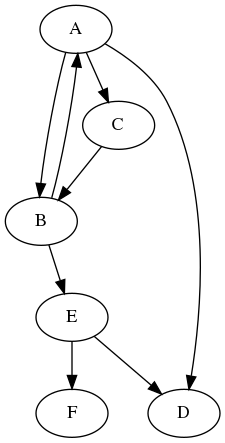
\includegraphics[width=.25\linewidth]{./img/graphe.png}
\end{center}

Le parcours sur ce graphe en partant de "A" devrait donner: A-B-E-F-D-C


\section{Behaviour trees:}
\label{sec-4}

Un behaviour tree (BT) est un outil permettant de concevoir un comportement pour un agent autonome, il permet également de l'exécuter. Pour évaluer un BT, on lance un parcours du graphe depuis la racine du graphe, parcours que l'on va appeler \emph{tick}. Chaque noeud va donc évaluer ses enfants selon des règles qui sont associées au type de noeud auquel ils appartiennent. Pour chaque évaluation, un noeud devra retourner à son père son état qui peut être Succès, Échec ou En Cours.

\clearpage

\noindent
Les \textbf{noeuds composites}, ce sont les noeuds de parcours du graphe, ils parcourent leurs enfants selon leurs règles et retournent leur état selon l'état de leurs enfants. La plupart des noeuds évaluent leurs enfants de gauche à droite. Les noeuds composites de la bibliothèque \emph{py-trees} sont les suivantes:
\begin{itemize}
\item \verb~Sequence~: Il évalue l'enfant suivant uniquement si le précédent retourne Succès. Sinon il retourne l'état du dernier enfant. Il ne retourne Succès que lorsque tous les enfants ont réussi.
\item \verb~Selector~: Il retourne Succès dès le premier enfant qui retourne Succès. Si aucun enfant ne retourne Succès, il retourne Échec.
\item \verb~Parallel~: Il évalue tous ses enfants en même temps. Dans son comportement de base, si tous les enfants réussissent, il retourne Succès. Sinon il retourne En Cours.
\item \verb~Chooser~: Vous n'en aurez fort probablement pas besoin.
\end{itemize}

\noindent
Les \textbf{noeuds d'exécution}, ce sont les noeuds qui interagissent avec le modèle, ils éxécutent une fonction du modèle. La bibliothèque \emph{py-trees} ne proposant pas d'implémentation de ces noeuds, utilisez le noeuds Action se trouvant dans \emph{toolkit.py.} Ce noeud permet le lancement d'une fonction avec au plus un argument. Si la fonction retourne \verb~True~, le noeud retourne Succès. Si la fonction retourne \verb~False~, le noeud retourne Échec. Si la fonction retourne \verb~None~, la fonction retourne En Cours.

\noindent
Il existe également les \textbf{noeuds décorateurs}, ce sont des noeuds ne prenant qu'un seul enfant, et qui changent l'état de retour de cet enfant selon des règles qui ont été définies pour ce décorateur. Par exemple, la bibliothèque \emph{py-trees} propose le décorateur \verb~Inverter~ qui inverse l'état entre Succès et Échec.

\noindent
Pour tout renseignement supplémentaire, la documentation de \emph{py-trees} se trouve à l'adresse suivante: \url{https://py-trees.readthedocs.io}

\noindent
Pour vous familiariser avec la bibliothèque, codez le comportement suivant avec l'aide des fichiers \emph{trameBT.py} et \emph{robot.py}:

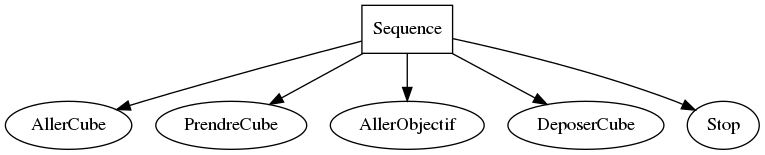
\includegraphics[width=\linewidth]{./img/robot.png}
% Emacs 25.2.2 (Org mode 8.2.10)
\end{document}